\documentclass[12pt]{exam}

\newcommand{\course}{MTH 234 Summer 2021}
\newcommand{\qdate}{Surface Integrals} %PUT DATE HERE
\newcommand{\quiz}{Group Work} 

    \usepackage[top=1in, bottom=1in, left=.45in, right=.45in]{geometry}
    \usepackage{amsmath,amsthm,amssymb,amstext}
    \usepackage{enumerate,enumitem}
    \usepackage{tikz,float,graphicx}
    \usepackage{microtype}
    \usepackage{bm,tikz}
        \usetikzlibrary{calc}
    \usepackage{multicol}
    \usepackage{nicematrix}
    \usepackage{cleveref}
    \usepackage[framemethod=tikz]{mdframed}
    
    %\newcommand{\course}{MTH 234 Summer 2021}
    %\newcommand{\qdate}{Equations of lines and planes} %PUT DATE HERE
    %\newcommand{\quiz}{Group Work} 
    
    \newcommand{\R}{\mathbb{R}}
    
    \newcommand{\ba}{\bm{a}}
    \newcommand{\bb}{\bm{b}}
    \newcommand{\bc}{\bm{c}}
    \newcommand{\bi}{\bm{i}}
    \newcommand{\bj}{\bm{j}}
    \newcommand{\bk}{\bm{k}}
    \newcommand{\br}{\bm{r}}
    \newcommand{\bv}{\bm{v}}
    \newcommand{\gen}[1]{\left\langle #1 \right\rangle}

\newtheorem*{theorem}{Theorem}
\surroundwithmdframed[]{theorem}

\theoremstyle{definition}
    \newtheorem*{definition}{Definition}
    \surroundwithmdframed[]{definition}
    \newtheorem*{info}{Useful Information}
    \surroundwithmdframed[]{info}
\theoremstyle{remark}
    \newtheorem*{remark}{Remark}
    \surroundwithmdframed[]{remark}
    

%%%%%%%%%%%%%%%%%%%%%%%
% HEADER AND FOOTER
%%%%%%%%%%%%%%%%%%%%%%%
\pagestyle{headandfoot}
\firstpageheadrule
\runningheadrule
\firstpageheader{\course}{\quiz}{\qdate}
\runningheader{\course}{\quiz}{\qdate}
\runningfooter{}{}{}


\usepackage{color}
\shadedsolutions
\definecolor{SolutionColor}{rgb}{0.8,0.9,1}

\usepackage{pgfplots}
    \pgfplotsset{every axis/.append style={
                    axis x line=middle,    % put the x axis in the middle
                    axis y line=middle,    % put the y axis in the middle
                    axis line style={<->}, % arrows on the axis
                    xlabel={$x$},          % default put x on x-axis
                    ylabel={$y$},          % default put y on y-axis
                    grid=both,
                    %xtick={-4,...,-1,1,...,3},
                    %ytick={-1,1,}
    }}
    \pgfplotsset{compat=1.17}

\newcommand{\bif}{\quad\iff\quad}

\printanswers
%\noprintanswers

\begin{document}
\section*{\qdate}


\begin{enumerate}
    \item \textbf{Parametric Surfaces:}

        For a surface \(S\) given by
        \(
            \bm{r}(u,v)=\gen{x(u,v),y(u,v),z(u,v)},~(u,v)\in D
        \)
        The integral of \(f(x,y,z)\) over \(S\) is given by
        \[
            \boxed{\iint_S~f(x,y,z)~dS = \iint_{D}~f(\br{r}(u,v))~|\bm{r}_u\times \bm{r}_v|~dA}
        \]
    \item \(\bm{z=g(x,y)}\)

        For \(S\) given by \(z=g(x,y)\) with \((x,y)\in D\), 
        \[
            \boxed{\iint_S~f(x,y,z)~dS = \iint_D~f(x,y,g(x,y))~\sqrt{ \left(\pd{z}{x}\right)^2+\left(\pd{z}{y}\right)^2+1}~dA}
        \]
    \item \textbf{Vector Fields}

        If \(\bm{F}\) is a continuous vector field on an oriented surface \(S\) with unit normal vector \(\bm{n}\) then 
        \begin{align*}
        \iint_S\bm{F}\cdot~d\bm{S} & = \iint_S~\bm{F}\cdot \bm{n}~dS\\
            & = \iint_{D}~\bm{F}\cdot\left(\bm{r}_u\times\bm{r}_v\right)~dA \quad \text{(If $S$ is given by \(r(u,v)\))}
        \end{align*}
            
    
\end{enumerate}

~

\begin{questions}

% 16.7 #11
\question Evaluate \(\iint_S~x^2z^2~dS\) where \(S\) is the part of the cone 
\(z^2=x^2+y^2\) that lies between the planes \(z=1\) and \(z=3\).
\ifprintanswers
        \begin{solution}
            Since \(z\) is always positive between \(1\) and \(3\), we may rewrite the surface as 
            \[
                z=\sqrt{x^2+y^2}.
            \]
            Note that 
            \begin{align*}
                \sqrt{\pd{z}{x}^2+\pd{z}{y}^2+1} & = \sqrt{\frac{x^2}{x^2+y^2}+\frac{y^2}{x^2+y^2}+1}\\
                    &= \sqrt{2}
            \end{align*}
            So our integral becomes 
            \begin{align*}
                \iint_D~x^2\left(\sqrt{x^2+y^2}\right)^2~\sqrt{2}~dA & = \sqrt{2}\iint_{D}x^4+x^2y^2~dA
            \end{align*}
            What is \(D\)?

            When \(z=1\) we have \(x^2+y^2=1\) and when \(z=3\) \(x^2+y^2=9\). 
            So \(D\) is the area in the \(xy\)-plane between the circles of radius \(1\) and \(3\) both centered at the origin. Shown in green below.
            \begin{center}
                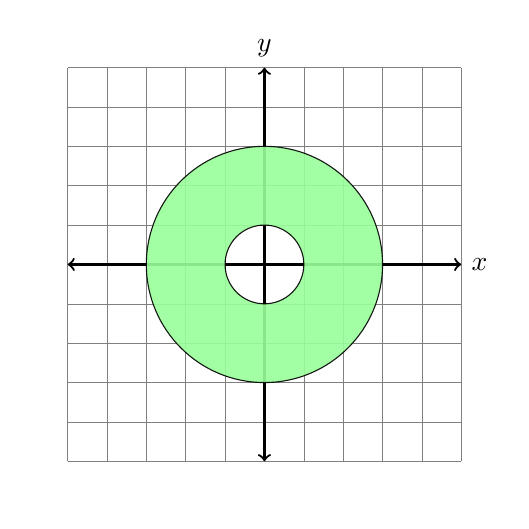
\begin{tikzpicture}[scale=.5]
                    \draw[white,fill=white] (-6,-6) rectangle (6,6);
                    \draw[very thin,gray] (-5,-5) grid[step=1] (5,5);
                    \draw[<->,thick] (-5,0)--(5,0) node[right] {$x$};
                    \draw[<->,thick] (0,-5)--(0,5) node[above] {$y$};
                    \draw[fill=green!40,even odd rule,opacity=.9] (0,0) circle (1) (0,0) circle (3);
                \end{tikzpicture}
            \end{center}
            This is clearly easier if we use polar coordinates, i.e. \(x=r\cos\theta\) and \(y=r\sin\theta\).
            \begin{align*}
            \sqrt{2}\iint_{D}x^4+x^2y^2~dA & = \sqrt{2}\int_0^{2\pi}\int_1^3~\left(r^4\cos^4\theta+r^4\cos^2\theta\sin^2\theta\right)r~dr~d\theta\\
            &= \sqrt{2}\int_0^{2\pi}\int_1^3 r^5\cos^2\theta\left(\cos^2\theta+\sin^2\theta\right)~dr~d\theta\\
            & = \sqrt{2}\int_{0}^{2\pi}\cos^2\theta \int_1^3 r^5~dr~d\theta\\
                & = \left(\frac{364}{3}\right)\sqrt{2}\pi
            \end{align*}
        \end{solution}
    \else
        \vfill
    \fi

\newpage 

% 16.7 #9
\question Evaluate \(\iint_S~yz~dS\) where \(S\) is the surface with parametric equations
\[
    x=u^2,~~y=u\sin v,~~z=u\cos v
\]
\[
    0\le u \le 1,~~0\le v\le \pi/2
\]
\ifprintanswers
        \begin{solution}
            \(S\) is given by 
            \[
                \bm{r}(u,v)=\gen{u^2,u\sin v,u\cos v}.
            \]
            Then 
            \begin{align*}
                \bm{r}_u\times \bm{r}_v & = \gen{2u,\sin v,\cos v}\times \gen{0,u\cos v,-u\sin v}\\
                    & 
            \end{align*}
        \end{solution}
    \else
        \vfill
    \fi

% Webwork: Problem 4
\question Find the mass of the surface \(S\), given by \(x=3z^2-4y\), \(0\le y \le 1\), \(0\le z \le 1\), if its density function is \(\rho(x,y,z)=2z\).
\ifprintanswers
        \begin{solution}
            
                Since the surface is of the form \(x=g(y,z)\) we use
                \begin{align*}
                    \iint_S~\rho\left(g(y,z),y,z\right)~\sqrt{\left(\pd{y}{x}\right)^2+\left(\pd{z}{x}\right)^2+1}~dS & = \int_0^1\int_0^1~2z\sqrt{17+36z^2}~dz~dy\\
                        & = \left(\frac{2}{3}\right) \left(\frac{1}{36}\right) \left((17+36)^{3/2} - 17^{3/2} \right)\\
                        & \approx 5.84728
                \end{align*}
        \end{solution}
    \else
        \vfill
    \fi

    \newpage

\question Evaluate \(\iint_S\left(-xy\bi-yz\bj+zx\bk\right)\cdot~d\bm{S}\) where 
\(S\) is the part of the parabaloid \(z=1-x^2-y^2\) that lies above the square \(0\le x \le 2\), \(0\le y \le 4\), and has upward orientation.
\ifprintanswers
        \begin{solution}
        \end{solution}
    \else
        \vfill
    \fi

\question Evaluate \(\iint_S~\bm{F}\cdot ~d\bm{S}\) where
\[
    \bm{F}(x,y,z) = xze^y\bi + xze^y \bj +z \bk,
\]
and \(S\) is the part of the plane \(x+y+z=1\) in the first octant and has downward orientation.
\ifprintanswers
        \begin{solution}
        \end{solution}
    \else
        \vfill
    \fi 




\end{questions}

\end{document}

% soln : Question environment
    \ifprintanswers
        \begin{solution}
        \end{solution}
    \else
        \vfill
    \fi